\label{chap.8}
\section{Introduction}
This chapter evaluates the whole pipeline in the unified environment of Chapter~\ref{chap.4}. We ask whether knowing the demand of the next interval helps allocation, whether the forecast helps the learned controller, how the controllers behave over the whole city, and what a Digital Twin adds to the work. We then describe the Digital Twin dataset and its what-if scenarios, and finish by testing the surrogate environment against a packet-level simulator.

\section{Value of the Forecast}
\label{sec:forecast-value}
On the held-out week the retrained forecaster of Chapter~\ref{chap.6} has a mean squared error that is 18\%, 33\% and 31\% lower than persistence for eMBB, URLLC and mMTC. To see what this is worth for allocation, we ran the same expert rule with three kinds of knowledge about the next ten minutes: the current demand, the TGNN forecast, and the true next demand, which is an upper bound for any forecast. Table~\ref{tab:forecast-value} gives the result.

\begin{table}[htbp]
\centering
\caption{Reward of the expert rule with different knowledge of the next ten minutes, held-out week (default targets)}
\label{tab:forecast-value}
\footnotesize
\begin{tabular}{|>{\centering\arraybackslash}p{\dimexpr 0.121\textwidth-2\tabcolsep\relax}|>{\centering\arraybackslash}p{\dimexpr 0.121\textwidth-2\tabcolsep\relax}|>{\centering\arraybackslash}p{\dimexpr 0.121\textwidth-2\tabcolsep\relax}|>{\centering\arraybackslash}p{\dimexpr 0.121\textwidth-2\tabcolsep\relax}|>{\centering\arraybackslash}p{\dimexpr 0.121\textwidth-2\tabcolsep\relax}|>{\centering\arraybackslash}p{\dimexpr 0.121\textwidth-2\tabcolsep\relax}|>{\centering\arraybackslash}p{\dimexpr 0.121\textwidth-2\tabcolsep\relax}|>{\centering\arraybackslash}p{\dimexpr 0.121\textwidth-2\tabcolsep\relax}|}
\hline
\textbf{Cells} & \textbf{Equal split} & \textbf{Current demand} & \textbf{TGNN forecast} & \textbf{True next demand} & \textbf{Forecast minus current (95\% CI)} & \textbf{Days better} & \textbf{Gap recovered} \\ \hline
9 & 0.785 & 0.794 & 0.825 & 0.945 & +0.030 $\pm$ 0.008 & 7/7 & 20\% \\ \hline
25 & 0.750 & 0.775 & 0.804 & 0.920 & +0.029 $\pm$ 0.006 & 7/7 & 20\% \\ \hline
49 & 0.728 & 0.758 & 0.788 & 0.902 & +0.029 $\pm$ 0.004 & 7/7 & 20\% \\ \hline
100 & 0.735 & 0.765 & 0.794 & 0.908 & +0.029 $\pm$ 0.004 & 7/7 & 20\% \\ \hline
\end{tabular}
\end{table}

\begin{figure}[htbp]
\centering
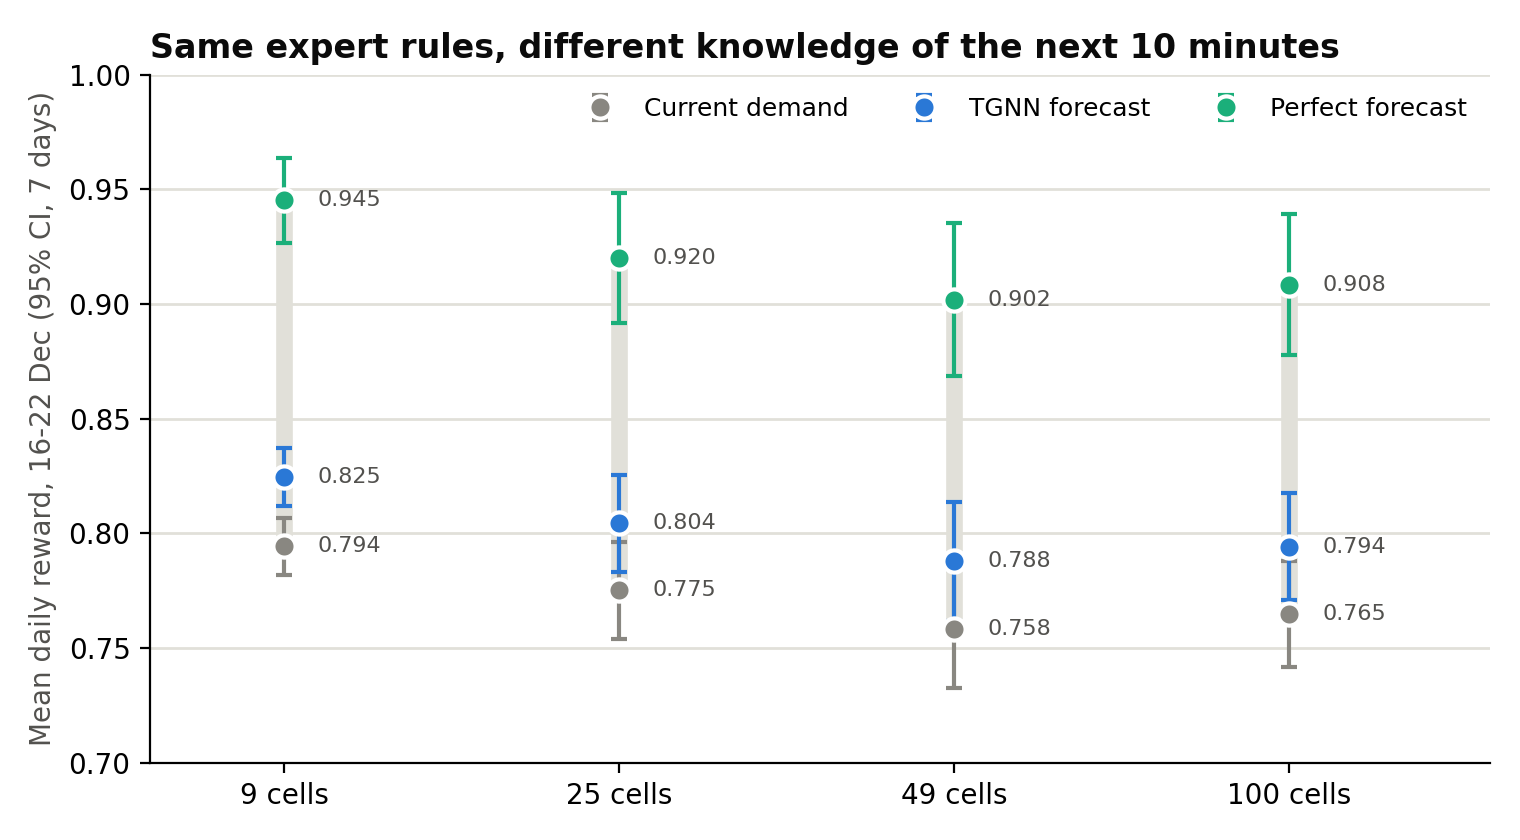
\includegraphics[width=0.85\textwidth,keepaspectratio]{unified_prediction_value.png}
\caption{Value of prediction for the expert rule at four network sizes}
\label{fig:forecast-value}
\end{figure}

The forecast improves the expert rule by about 0.03 in reward at every network size and on all seven test days, with intervals of about 0.004 to 0.008. It closes about one fifth of the gap to perfect knowledge. An earlier estimate of 0.05 came from two test days and a forecaster trained on five days. With 39 training days and a whole week of testing, the benefit is smaller but better established. Using the value of the previous day at the same time as a forecast does not work: its mean reward is 0.74 to 0.78 at every size, which is below that of current demand.

\section{The Forecast and the Learned Controller}
\label{sec:forecast-marl}
We also gave the forecast to the MARL controller as an extra input. Table~\ref{tab:forecast-marl} shows that at this training budget, with three seeds, it made no reliable difference. Giving the controller the true next-interval demand did not help either.

\begin{table}[htbp]
\centering
\caption{MARL with and without forecast input (25 cells, three seeds, mean $\pm$ sample standard deviation)}
\label{tab:forecast-marl}
\footnotesize
\begin{tabular}{|>{\centering\arraybackslash}p{\dimexpr 0.300\textwidth-2\tabcolsep\relax}|>{\centering\arraybackslash}p{\dimexpr 0.170\textwidth-2\tabcolsep\relax}|}
\hline
\textbf{Input to the MARL controller} & \textbf{Held-out reward} \\ \hline
No forecast & $0.778\pm0.048$ \\ \hline
Forecast from the first (5-day) TGNN & $0.765\pm0.051$ \\ \hline
Forecast from the retrained TGNN & $0.772\pm0.073$ \\ \hline
True next-interval demand & $0.762\pm0.057$ \\ \hline
\end{tabular}
\end{table}

\begin{figure}[htbp]
\centering
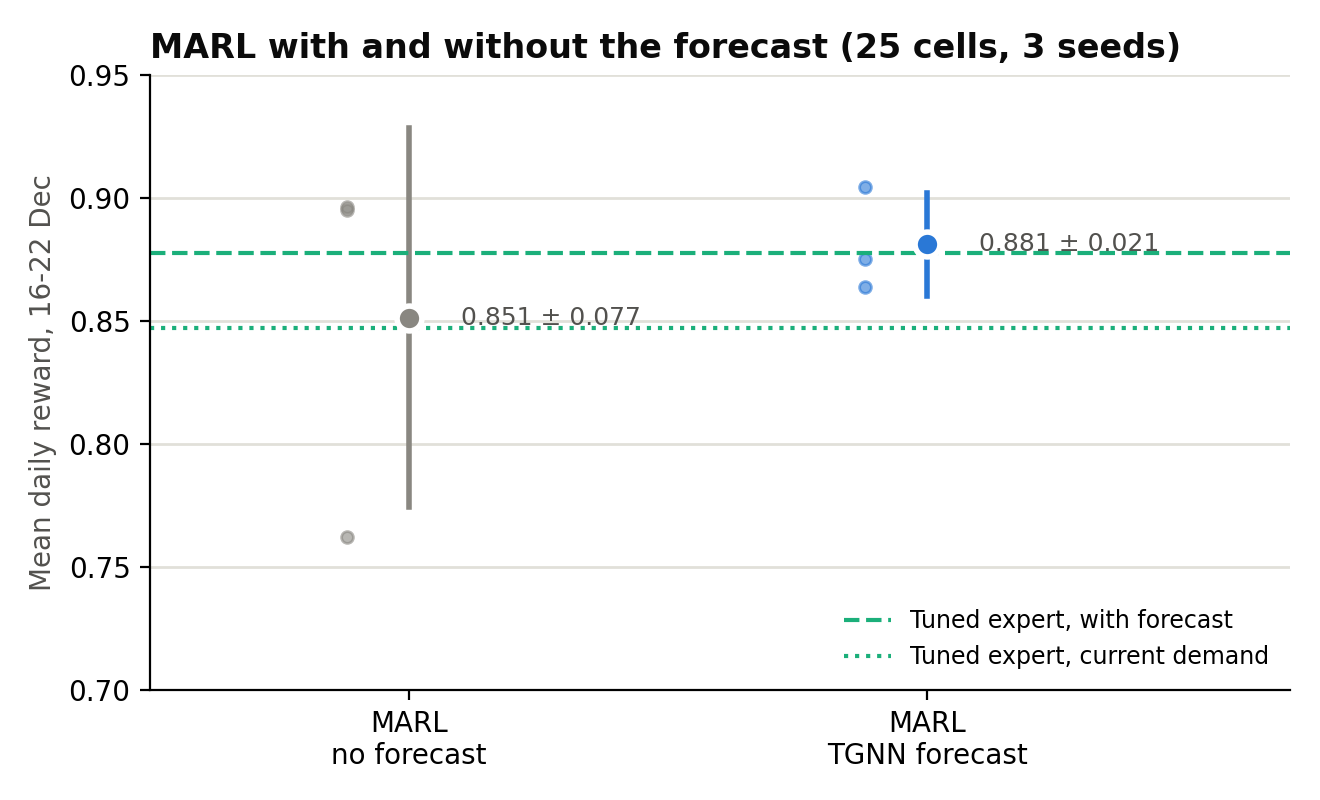
\includegraphics[width=0.8\textwidth,keepaspectratio]{unified_forecast_ablation.png}
\caption{Learned controller with and without the forecast}
\label{fig:forecast_for_marl}
\end{figure}

The three rewards differ by less than their sample standard deviations of 0.05 to 0.06, so the experiment shows neither a clear gain nor a clear loss. Under shifted traffic the effect on the learned policy even changes sign (Section~\ref{sec:marl_shift}). We therefore claim that forecasting helps the rule-based controller, and we have not shown that it helps the learned one. The forecast is still useful: the Digital Twin gate of Section~\ref{sec:gate} uses it to predict the outcome of a proposed allocation.

\section{Controllers Across the Whole City}
\label{sec:city-controllers}
We ran the three controllers of the Slice Twin monitor (Chapter~\ref{chap.9}) on all 10{,}000 Milan cells for one day, Wednesday 6 November 2013, with scripted incidents. Static divides the capacity equally. Reactive applies the expert rule to the current demand. Predictive applies it to the city-wide forecast. The forecaster was not trained on this day.

\begin{table}[htbp]
\centering
\caption{Controllers on all 10{,}000 cells, Wednesday 6 November 2013 (reward of the whole city, the dense block and the outer city)}
\label{tab:city-controllers}
\footnotesize
\begin{tabular}{|>{\centering\arraybackslash}p{\dimexpr 0.194\textwidth-2\tabcolsep\relax}|>{\centering\arraybackslash}p{\dimexpr 0.194\textwidth-2\tabcolsep\relax}|>{\centering\arraybackslash}p{\dimexpr 0.194\textwidth-2\tabcolsep\relax}|>{\centering\arraybackslash}p{\dimexpr 0.194\textwidth-2\tabcolsep\relax}|>{\centering\arraybackslash}p{\dimexpr 0.194\textwidth-2\tabcolsep\relax}|}
\hline
\textbf{Controller} & \textbf{SLA met (eMBB / URLLC / mMTC)} & \textbf{Whole city} & \textbf{Dense block} & \textbf{Outer city} \\ \hline
Static & 0.919 / 0.997 / 1.000 & 0.974 & 0.709 & 0.977 \\ \hline
Reactive & 0.975 / 0.711 / 0.568 & 0.839 & 0.735 & 0.840 \\ \hline
Predictive & 0.975 / 0.786 / 0.601 & 0.868 & 0.773 & 0.869 \\ \hline
\end{tabular}
\end{table}

In the dense block the Predictive controller scores highest (0.773 against 0.735 and 0.709), as in Section~\ref{sec:forecast-value}. Over the whole city, however, Static scores highest (0.974 against 0.868 and 0.839). Most cells are lightly loaded, and when URLLC and mMTC traffic is close to zero the rule gives those slices very little capacity, so they miss their targets when traffic comes back. The outer city has most of the cells, and this outweighs the benefit of forecasting. An earlier run reported 0.935 for the Predictive controller over the city. That came from over-allocation caused by a bias of the block-trained forecaster in the outer cells, and the table above replaces it. Since this is a single day, it shows how the controllers behave and does not rank them.

\section{The Digital Twin Dataset}
\label{sec:dt-dataset}
No public dataset contains topology, per-slice traffic, QoS metrics, SLA outcomes and allocation decisions together, so we generated one from the unified environment (\texttt{src/\allowbreak unified/\allowbreak twin\_\allowbreak dataset.py}). Each row is one cell in one 10-minute interval. The data is stored as Parquet files on the project drive, and summaries and samples are in the repository. We made two builds (Table~\ref{tab:dt-size}), with 393.6 million rows in total.

\begin{table}[htbp]
	\centering
	\caption{Size of the Digital Twin dataset}
	\label{tab:dt-size}
	\small
	\resizebox{\textwidth}{!}{%
	\begin{tabular}{|l|c|c|c|r|c|}
		\hline
		\textbf{Build} & \textbf{Cells} & \textbf{Days} & \textbf{Scenarios} & \textbf{Rows} & \textbf{Size} \\
		\hline
		Core year (central $20\times 20$ block) & 400 & 364 & 6 & 125{,}796{,}000 & 30.8 GB \\
		Full city (whole grid) & 10{,}000 & 62 & 3 & 267{,}810{,}000 & 40.5 GB \\
		\hline
		\textbf{Total} & & & & \textbf{393{,}606{,}000} & \\
		\hline
	\end{tabular}}
\end{table}

\paragraph{Provenance.}
The 62 recorded days are real Telecom Italia Milan data \cite{barlacchi2015}. The other days of the core year are bootstrapped from real days of the same weekday, with 20\% growth per year and a little random variation. The columns \texttt{source} and \texttt{source\_date} say whether a row is real or bootstrapped. Latency and jitter follow curves calibrated on the 6G RAN telemetry. The radio fields follow the 3GPP CQI table \cite{3gpp38214} and the power follows the EARTH base-station model \cite{auer2011}. The slice mapping, the industrial zones, the per-user rates and the packet sizes are our own assumptions.

\paragraph{Structure.}
Each row has 122 columns. Twenty are for identity and calendar, 3 for control, 8 for events and state, 11 for radio and capacity, 6 for the neighbourhood and 3 for energy. There are 63 per-slice fields (21 for each slice, including the demand 10, 30 and 60 minutes ahead as forecasting targets), 2 for the reward and 6 for noisy telemetry. Appendix~\ref{app:columns} lists all of them.

\paragraph{Validation.}
We ran all six scenarios for three days before the full build and checked five things. All scenarios have the same interval and cell rows. Traffic is conserved under energy saving, since the traffic that sleeping cells hand over equals what the neighbours receive. The industrial and massive-IoT multipliers are applied exactly. 1.0\% of the telemetry is missing, as designed. The 10- and 60-minute targets equal the demand of the same cell one and six rows later. These are automated tests in the repository. They show that the generator is consistent with itself, not that it agrees with a packet-level simulator.

\section{What-if Scenarios}
\label{sec:scenarios}
All scenarios share the same days, the same behaviour policy and the same random noise, so any difference between two scenarios comes from the scenario. Table~\ref{tab:scenarios} gives the results for the core year.
\begin{table}[htbp]
	\centering
	\caption{Scenarios of the core year}
	\label{tab:scenarios}
	\footnotesize
	\begin{tabular}{|p{2.3cm}|p{4.6cm}|p{3.4cm}|p{1.3cm}|p{1.8cm}|}
		\hline
		\textbf{Scenario} & \textbf{What changes} & \textbf{SLA met (eMBB / URLLC / mMTC)} & \textbf{Reward} & \textbf{Energy (MWh)} \\
		\hline
		baseline & Recorded traffic, no incidents & 0.704 / 0.731 / 0.651 & 0.763 & 3{,}473 \\
		\hline
		events & Adds flash crowds, outages, interference, URLLC bursts, mMTC storms, capacity degradation & 0.703 / 0.730 / 0.651 & 0.763 & 3{,}473 \\
		\hline
		growth\_6g & eMBB $\times$1.3, URLLC $\times$2, mMTC $\times$3 & 0.553 / 0.696 / 0.610 & 0.688 & 3{,}648 \\
		\hline
		energy\_saving & Quiet cells sleep 01:00--05:00 and hand traffic to neighbours & 0.703 / 0.737 / 0.659 & 0.766 & 3{,}435 \\
		\hline
		industrial\_urllc & Industrial cells: URLLC $\times$4 in weekday shifts & 0.693 / 0.723 / 0.646 & 0.756 & 3{,}481 \\
		\hline
		massive\_iot & mMTC $\times$10, a further $\times$3 at the start of each hour & 0.554 / 0.710 / 0.524 & 0.660 & 3{,}628 \\
		\hline
	\end{tabular}
\end{table}

The scaled-traffic scenarios behave as intended. growth\_6g lowers the eMBB compliance from 0.704 to 0.553, and massive\_iot lowers the mMTC compliance from 0.651 to 0.524 and uses the most energy. The events scenario is almost the same as the baseline because over 99.8\% of its rows have no event. The effect only shows when the rows are grouped by event type (Table~\ref{tab:events}).

\begin{table}[htbp]
	\centering
	\caption{Effect of each injected event (core year, events scenario)}
	\label{tab:events}
	\small
	\begin{tabular}{|l|r|c|c|}
		\hline
		\textbf{Event} & \textbf{Rows} & \textbf{SLA met (eMBB / URLLC / mMTC)} & \textbf{Reward} \\
		\hline
		none & 20{,}932{,}659 & 0.704 / 0.730 / 0.651 & 0.763 \\
		flash crowd & 19{,}740 & 0.217 / 0.683 / 0.598 & 0.532 \\
		cell outage & 985 & 0.000 / 0.095 / 0.019 & 0.019 \\
		interference spike & 8{,}883 & 0.577 / 0.697 / 0.629 & 0.704 \\
		URLLC burst & 814 & 0.608 / 0.510 / 0.575 & 0.631 \\
		mMTC storm & 1{,}966 & 0.658 / 0.730 / 0.344 & 0.679 \\
		capacity degradation & 953 & 0.323 / 0.710 / 0.647 & 0.578 \\
		\hline
	\end{tabular}
\end{table}

\paragraph{Energy saving across the city.} We also ran the energy-saving scenario on the whole city for 62 days (Table~\ref{tab:energy}). When lightly loaded cells sleep from 01:00 to 05:00, night-time energy drops by 19.6\%, from 1{,}983 MWh to 1{,}593 MWh, and total energy over the period drops by 3.2\%. The price is that the URLLC compliance of the awake cells falls from 0.761 to 0.720, because their mean load rises from 0.045 to 0.066. The saving has to be read together with this loss of QoS.

\begin{table}[htbp]
	\centering
	\caption{Night-time sleep across the city (01:00 to 05:00, 62 days)}
	\label{tab:energy}
	\small
	\begin{tabular}{|l|c|c|}
		\hline
		\textbf{Measure} & \textbf{Baseline} & \textbf{Energy saving} \\
		\hline
		Night-time energy (MWh) & 1983 & 1593 (19.6\% lower) \\
		Night cell-intervals asleep & 0\% & 47.6\% \\
		SLA met, awake cells (eMBB / URLLC / mMTC) & 0.983 / 0.761 / 0.724 & 0.976 / 0.720 / 0.693 \\
		Mean load of awake cells & 0.045 & 0.066 \\
		\hline
	\end{tabular}
\end{table}

\section{The Digital Twin as an Approval Gate}
\label{sec:gate}
A Digital Twin is only useful if it can check a decision before the decision is applied, and the unified environment now has a gate that does this. Before a cell's allocation is applied, the twin predicts the outcome of the next interval for the proposed allocation and for a safe fallback. It uses the QoS model of the environment and the TGNN forecast of the demand in that interval. The fallback is the expert rule tuned on the training days. The proposal is approved if its predicted reward is at least that of the fallback, and otherwise the fallback is applied. The gate works cell by cell.

We measured the gate on the held-out week with controllers whose proposals are sometimes bad, as when a learning agent explores online. These were the trained MARL actor with Gaussian noise of standard deviation $\sigma$ added to its logits, and an equal split. Table~\ref{tab:gate} gives the reward with and without the gate.

\begin{table}[htbp]
\centering
\caption{Effect of the approval gate on the held-out week (25 cells, mean over the three MARL seeds)}
\label{tab:gate}
\footnotesize
\begin{tabular}{|>{\centering\arraybackslash}p{\dimexpr 0.300\textwidth-2\tabcolsep\relax}|>{\centering\arraybackslash}p{\dimexpr 0.170\textwidth-2\tabcolsep\relax}|>{\centering\arraybackslash}p{\dimexpr 0.170\textwidth-2\tabcolsep\relax}|>{\centering\arraybackslash}p{\dimexpr 0.170\textwidth-2\tabcolsep\relax}|}
\hline
\textbf{Controller} & \textbf{Reward without gate} & \textbf{Reward with gate} & \textbf{Proposals approved} \\ \hline
MARL, logit noise $\sigma= 0$ & 0.900 & 0.898 & 72\% \\ \hline
MARL, logit noise $\sigma= 0.5$ & 0.805 & 0.876 & 7\% \\ \hline
MARL, logit noise $\sigma= 1.0$ & 0.707 & 0.877 & 3\% \\ \hline
MARL, logit noise $\sigma= 2.0$ & 0.574 & 0.877 & 1\% \\ \hline
Equal split & 0.750 & 0.879 & 2\% \\ \hline
\end{tabular}
\end{table}

The gate has two sides. For a good controller ($\sigma=0$) it gives nothing: the reward is the same to within 0.003, and the gate still rejects about a quarter to a third of the proposals. For degraded controllers it recovers almost everything that was lost and brings each case back to the reward of the fallback alone (0.8775). So the gate is a safety measure and not an improvement. It stops the result from dropping below the fallback when a proposal is poor, and how well it works depends on how good the twin's prediction is. Our twin uses the same QoS model as the environment it is tested in, so this experiment cannot tell us how accurate the gate would be on a real network.

\section{Checking the Surrogate Against a Packet-Level Simulator}
\label{sec:simu5g}
The QoS model of our environment is a calibrated surrogate. To test it against a packet-level simulator we ran a load sweep in Simu5G 1.7.0 (OMNeT++ 6.4, INET 4.7), with one gNodeB and ten UEs receiving downlink UDP traffic in messages of 1000 bytes. The offered load went from 11\% to 125\% of the measured capacity of 56.1 Mbps, with three repetitions per point. Table~\ref{tab:simu5g_sweep} and Figure~\ref{fig:simu5g_sweep} show the delay.

\begin{table}[htbp]
\centering
\caption{Simu5G load sweep (10 UEs, one gNodeB, downlink capacity 56.1 Mbps, 1000-byte messages, 6 s, mean of three repetitions)}
\label{tab:simu5g_sweep}
\footnotesize
\begin{tabular}{|>{\centering\arraybackslash}p{\dimexpr 0.300\textwidth-2\tabcolsep\relax}|>{\centering\arraybackslash}p{\dimexpr 0.170\textwidth-2\tabcolsep\relax}|>{\centering\arraybackslash}p{\dimexpr 0.170\textwidth-2\tabcolsep\relax}|>{\centering\arraybackslash}p{\dimexpr 0.170\textwidth-2\tabcolsep\relax}|}
\hline
\textbf{Utilisation} & \textbf{Median delay (ms)} & \textbf{95th-percentile delay (ms)} & \textbf{Received (Mbps)} \\ \hline
0.11 & 4.5 & 5.0 & 6.0 \\ \hline
0.21 & 4.5 & 4.9 & 12.0 \\ \hline
0.36 & 4.4 & 5.0 & 20.0 \\ \hline
0.54 & 4.5 & 5.0 & 30.0 \\ \hline
0.68 & 4.7 & 6.9 & 38.0 \\ \hline
0.78 & 4.6 & 6.8 & 44.0 \\ \hline
0.86 & 6.0 & 6.8 & 48.0 \\ \hline
0.93 & 6.1 & 434.5 & 50.5 \\ \hline
1.00 & 5.9 & 1376.2 & 50.1 \\ \hline
1.07 & 5.8 & 780.8 & 50.7 \\ \hline
1.25 & 11.1 & 211.9 & 55.6 \\ \hline
\end{tabular}
\end{table}

\begin{figure}[htbp]
\centering
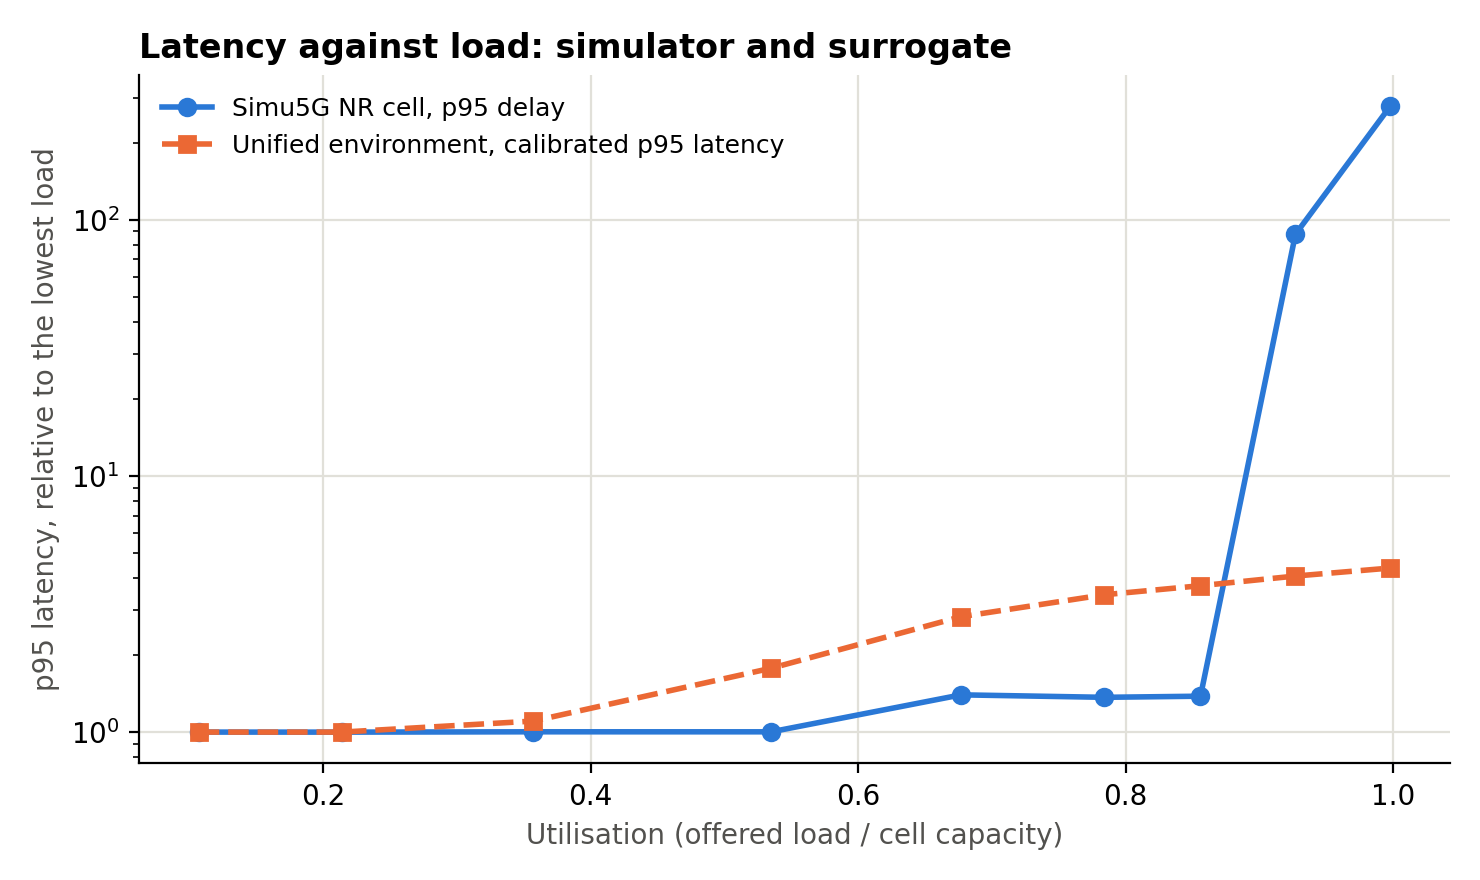
\includegraphics[width=0.8\textwidth,keepaspectratio]{simu5g_latency_vs_load.png}
\caption{Delay against load: Simu5G and the surrogate of the environment (normalised)}
\label{fig:simu5g_sweep}
\end{figure}

The two models agree on the ordering: the rank correlation of the normalised 95th-percentile delay between Simu5G and our surrogate is 0.93. They do not agree on the shape. In Simu5G the delay stays flat at about 5 ms until the load reaches about 93\% of capacity, and then it jumps, to 434 ms at 93\% and above one second at full load. Our surrogate rises slowly from 53\%, and the load at which its 95th-percentile delay doubles is 68\% rather than 93\%. The surrogate is therefore more cautious than the simulator at moderate load and far too optimistic beyond saturation. The 5 ms floor in the sweep comes from the scheduling of the simulator. We read this as a check of shape and ranking, not as a calibration of absolute values.

Because the controllers were developed on the surrogate, we repeated the evaluation on a latency curve with the shape of the Simu5G sweep (flat, then a cliff at capacity). Table~\ref{tab:simu5g_eval} gives the result. The ranking of the methods is the same as on the default curve: the forecast-fed rule beats the current-demand rule, and the learned controllers, which were not retrained, score about 0.95, above the rule tuned on this curve (0.942) and close to the rule that is given the true next demand (0.957). MAPPO retrained on this curve (three seeds) reaches 0.969, above that rule as well. The ordering of the controllers therefore does not depend on the smooth shape of the surrogate.

\begin{table}[htbp]
\centering
\caption{Controllers on the Simu5G-shaped latency curve (25 cells, held-out week)}
\label{tab:simu5g_eval}
\footnotesize
\begin{tabular}{|>{\centering\arraybackslash}p{\dimexpr 0.300\textwidth-2\tabcolsep\relax}|>{\centering\arraybackslash}p{\dimexpr 0.170\textwidth-2\tabcolsep\relax}|>{\centering\arraybackslash}p{\dimexpr 0.170\textwidth-2\tabcolsep\relax}|}
\hline
\textbf{Controller} & \textbf{Runs} & \textbf{Reward} \\ \hline
Equal split & 1 & 0.814 \\ \hline
Expert rule, untuned, current & 1 & 0.909 \\ \hline
Expert rule, tuned under this curve, current & 1 & 0.913 \\ \hline
Expert rule, untuned, forecast & 1 & 0.940 \\ \hline
Expert rule, tuned under this curve, forecast & 1 & 0.942 \\ \hline
Expert rule on the true next demand, untuned & 1 & 0.957 \\ \hline
IPPO, trained on the default curve, not retrained & 3 & $0.953\pm0.002$ \\ \hline
MAPPO, trained on the default curve, not retrained & 9 & $0.953\pm0.001$ \\ \hline
MAPPO, retrained under this curve & 3 & $0.968\pm0.000$ \\ \hline
DDPG-MARL, trained on the default curve, not retrained & 3 & $0.948\pm0.003$ \\ \hline
\end{tabular}
\end{table}

\section{The Role of the Digital Twin in This Work}
\label{sec:dt-role}
The Digital Twin has three roles in this work.
\begin{itemize}
    \item \textbf{Training and evaluation.} The unified environment combines real Milan traffic with modelled slice demand, allocation actions, QoS estimates, SLA outcomes and rewards.
    \item \textbf{Scenario generation.} The 393.6-million-row dataset, six what-if scenarios and automated consistency checks allow controlled evaluation under different conditions.
    \item \textbf{Approval gate.} Section~\ref{sec:gate} shows that the twin can reject poor proposals before they are applied, which protects the result from a degraded controller.
\end{itemize}
The main limit is that the QoS comes from a calibrated surrogate whose reference telemetry is itself simulated. The fall of the mean gap from 0.086 to 0.021 shows a good fit, not an independent validation, and the Simu5G sweep shows that the shape of the surrogate differs from a packet-level model. The twin therefore supports comparisons between controllers under assumptions that we state; it has not been validated for deployment decisions.

\section{Summary}
In the unified environment the TGNN forecast improves the expert rule by about 0.03 in reward at every network size and on all seven test days, which closes about one fifth of the gap to perfect knowledge. We have not shown that it improves the learned controller. Over the whole city the static split scores highest, because the rule starves the quiet slices, while in the dense block the predictive controller is best. The Digital Twin dataset supports six scenarios, among them an energy-saving policy that cuts night-time energy by 19.6\% at a URLLC cost on the awake cells. The twin also works as an approval gate that protects the result from poor proposals, and a Simu5G sweep shows that the surrogate agrees with the simulator on the order of delays but not on the shape of the delay curve.
